\documentclass{article}
\usepackage[pdftex]{graphicx}
\usepackage{hyperref}
\usepackage{amsmath}

\usepackage[utf8x]{inputenc}
\usepackage[T1]{fontenc}
\usepackage[frenchb]{babel}
\usepackage{float}
\usepackage{listings}

% for tables
\usepackage{booktabs}
\usepackage{multirow}

% dendogram
\usepackage{tikz}
\usepackage{subfig}


\begin{document}

\title{Introduction à la vision par ordinateur \\
TP1: Détection de visages}
\author{Romain Catajar - romain.catajar@student.ecp.fr}
\maketitle

\begin{abstract}
Présentation d'implémentations de différentes méthodes de détection de peau ou de visage et analyse des résultats. Le code a été réalisé avec l'aide de deux autres étudiants: Léo Hoummady et Thibault Kaspi.
\end{abstract}
% skip section 1 to 3
\stepcounter{section}
\stepcounter{section}
\stepcounter{section}
\section{Approche 1: Detection de la peau}
\subsection{Avant de commencer}
\begin{enumerate}
    \item Que pensez vous de ce type d'approches, que l'on pourra qualifier
d'approches colorimétriques, pour la détection de visages ? La détection
de la peau est-elle suffisante ? Quelles en sont les limites ?\\\\
Cette approche me semble être limité. En effet, même si on imagine pouvoir détecter parfaitement les pixels de peau, cela ne suffit pas a détecter le visage (le visage n'est pas forcement la seule peau apparaissant sur une image). De plus, je ne suis pas convaincu qu'une approche colorimetrique est suffisante pour detecter efficacement les pixels de peau. En effet la couleur des pixels de peau peux varier grandement d'une image a une autre en fonction de plusieurs critères (exposition et luminosité de la photo, ethnicité de la personne sur la photo, ...). Il me semble qu'une approche efficace devrait prendre en compte le contexte autour des pixels pour dire s'il s'agit de peau ou non (par exemple, en regardant le gradient de l'image, la couleur des pixels de peau devant a priori varier peu).\\

    \item Dans la mise en oeuvre de ce type d'approches, quelles sont les principales questions à se poser ? \\
    \begin{itemize}
        \item Qualité et variété des images utilisées (différents éclairages et couleurs de peau par exemple)
        \item Choix du modèle de séparation entre peau et non peau
        \item Choix de l'espace de couleur
    \end{itemize}
\end{enumerate}

\subsection{A vous de jouer}
\subsubsection{Base d'images}
J'ai construit une base de 78 images a partir du dataset \emph{Pratheepan Dataset}. Ces images sont ensuite séparées en deux groupe, un groupe "d'entrainement" de 52 images et un groupe de test de 26 images.

\subsubsection{Une première méthode simple}
Les résultats obtenues sont présenté dans le tableau ci dessous.

\begin{table}[h!]
\centering
\resizebox{\textwidth}{!}{%
\begin{tabular}{|c|c|c|c|c|}
\hline
\multirow{2}{*}{\textbf{Dataset}} & \multicolumn{2}{c|}{\textbf{Taux de bonne détection}} & \multicolumn{2}{c|}{\textbf{Taux de mauvaise détection}} \\ \cline{2-5}
 & \textit{Moyenne} & \textit{Ecart type} & \textit{Moyenne} & \textit{Ecart type} \\ \hline
\textit{Entrainement} & 0.87 & 0.14 & 0.28 & 0.20 \\ \hline
\textit{Test} & 0.91 & 0.09 & 0.16 & 0.15 \\ \hline
\end{tabular}%
}
\caption{Résultats de la méthode de Peer et Al.}
\label{peer-et-al}
\end{table}


 Globalement le taux de bonne détection est acceptable, mais celui de mauvaise détection est trop élevée (son ecart type egalement). La règle semble être trop permissive.




\begin{figure}[h!]
  \centering
  \subfloat[Résultat]{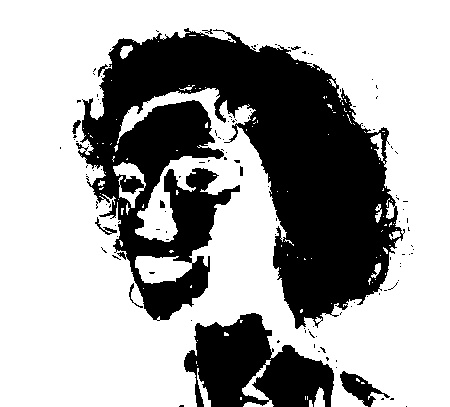
\includegraphics[width=0.4\textwidth]{img/peer1.jpg}\label{fig:f1}}
  \hfill
  \subfloat[Original]{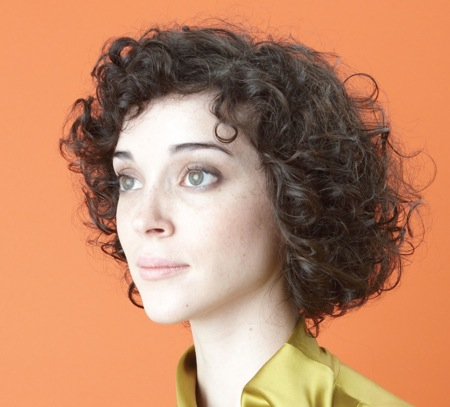
\includegraphics[width=0.4\textwidth]{img/peer2.jpg}\label{fig:f2}}
  \caption{Méthode de Peer et Al.: Exemple de mauvaise détection où l'arrière plan est detecté comme de la peau}
\end{figure}


\begin{figure}[h!]
  \centering
  \subfloat[Résultat]{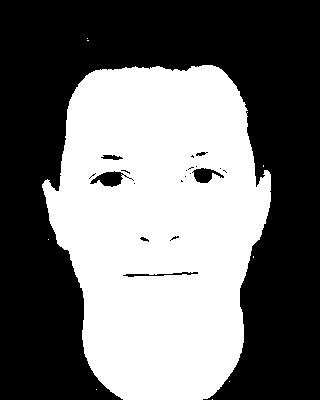
\includegraphics[width=0.4\textwidth]{img/peer3.jpg}\label{fig:f1}}
  \hfill
  \subfloat[Original]{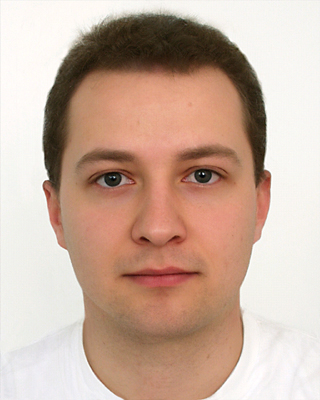
\includegraphics[width=0.4\textwidth]{img/peer4.jpg}\label{fig:f2}}
  \caption{Méthode de Peer et Al.: Exemple de bonne détection}
\end{figure}


\begin{figure}[h!]
  \centering
  \subfloat[Résultat]{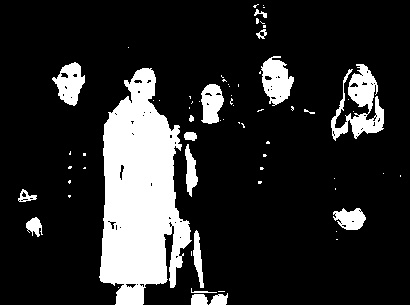
\includegraphics[width=0.4\textwidth]{img/peer5.jpg}\label{fig:f1}}
  \hfill
  \subfloat[Original]{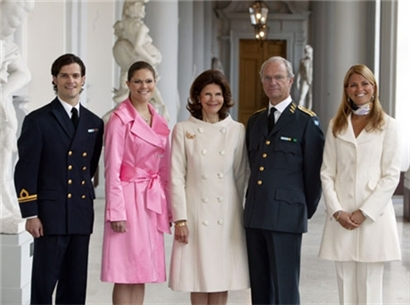
\includegraphics[width=0.4\textwidth]{img/peer6.jpg}\label{fig:f2}}
  \caption{Méthode de Peer et Al.: Exemple de mauvaise détection}
\end{figure}


\newpage
\subsubsection{Approche non paramétrique: Histogramme et modèle de peau}

J'ai construit les histogramme a partir du dataset d'entrainement pour les espaces RGB, LAB et HSV.
\begin{figure}[h!]
  \centering
  \subfloat[peau]{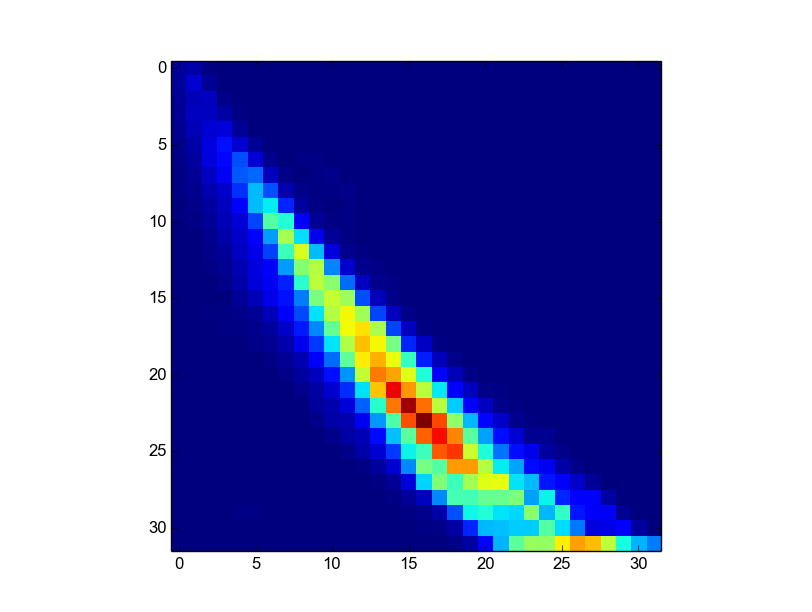
\includegraphics[width=0.47\textwidth]{img/rgb_skin.png}\label{fig:f1}}
  \hfill
  \subfloat[non peau]{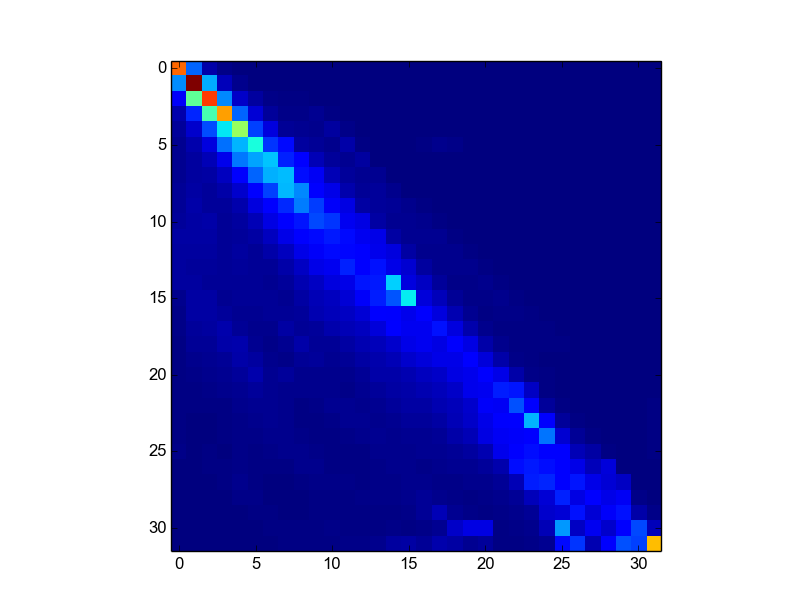
\includegraphics[width=0.47\textwidth]{img/rgb_not_skin.png}\label{fig:f2}}
  \caption{Histogramme RGB (sur R et G)}
\end{figure}

\begin{figure}[h!]
  \centering
  \subfloat[peau]{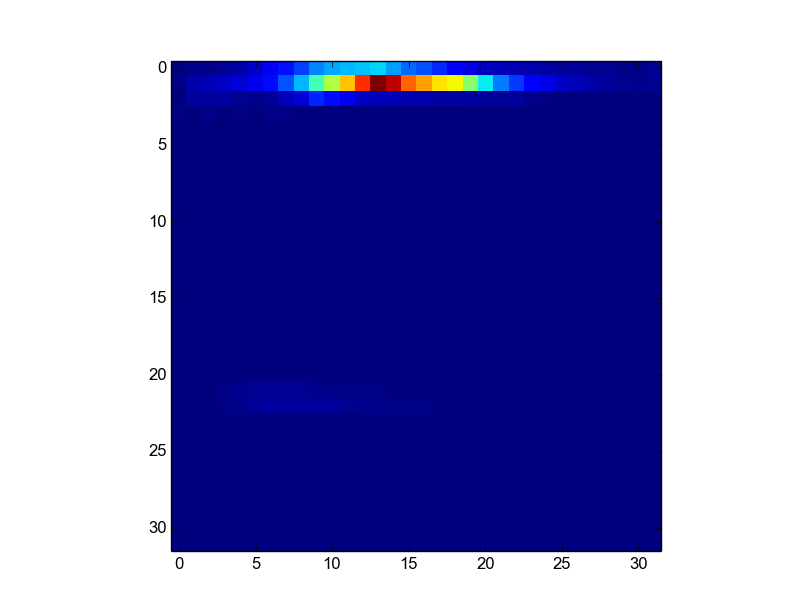
\includegraphics[width=0.47\textwidth]{img/hsv_skin.png}\label{fig:f1}}
  \hfill
  \subfloat[non peau]{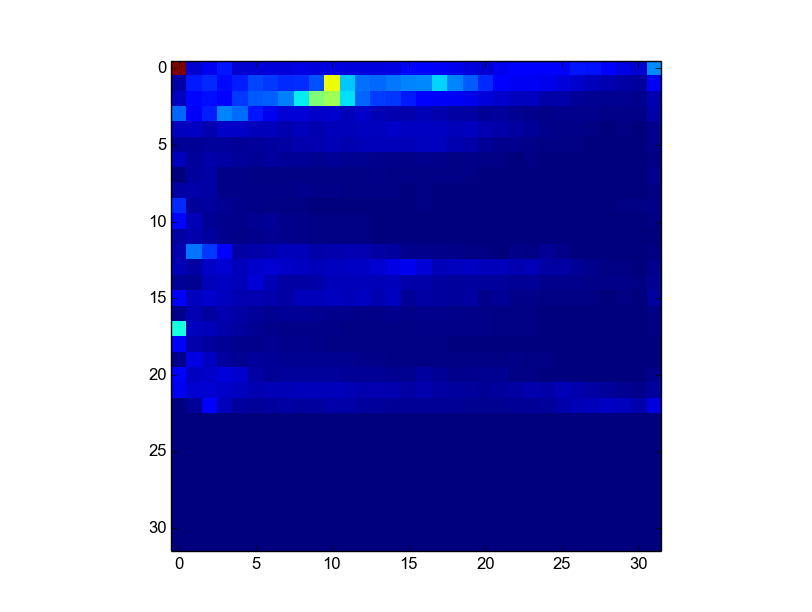
\includegraphics[width=0.47\textwidth]{img/hsv_not_skin.png}\label{fig:f2}}
  \caption{Histogramme HSV (sur H et S)}
\end{figure}

\begin{figure}[h!]
  \centering
  \subfloat[peau]{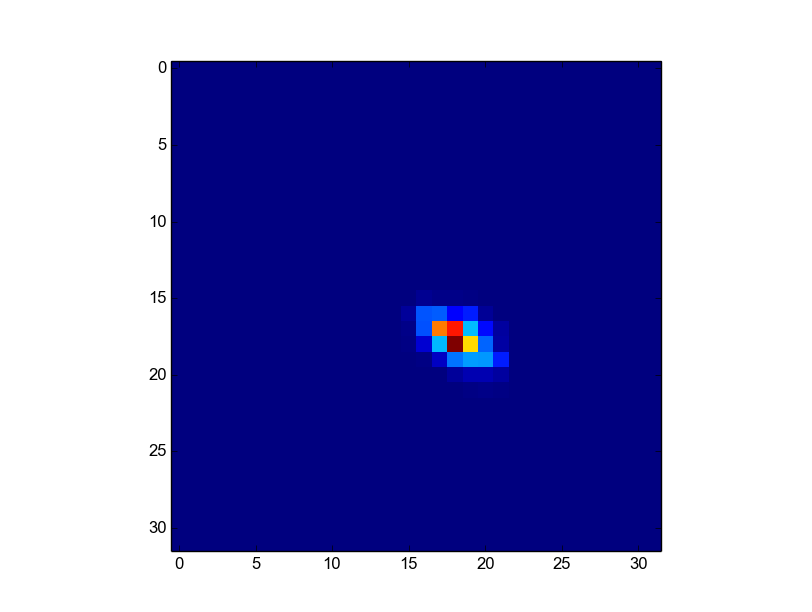
\includegraphics[width=0.47\textwidth]{img/lab_skin.png}\label{fig:f1}}
  \hfill
  \subfloat[non peau]{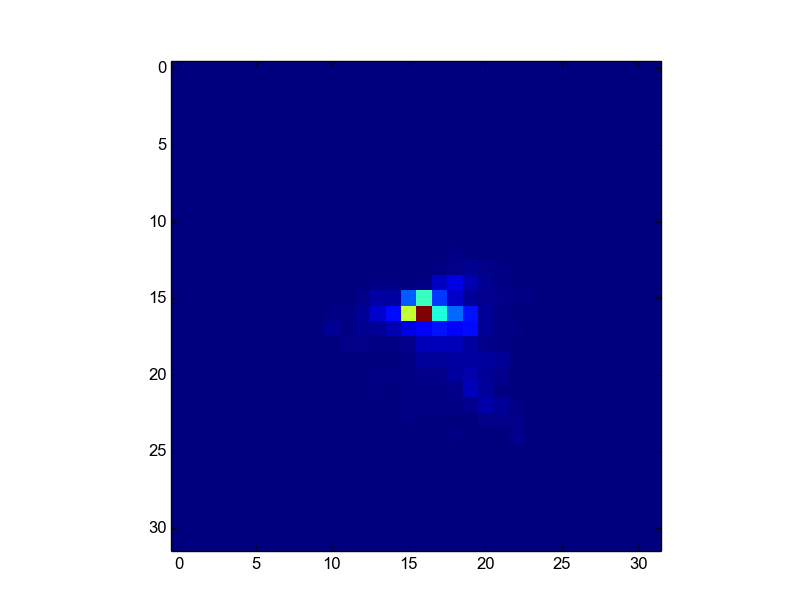
\includegraphics[width=0.47\textwidth]{img/lab_not_skin.png}\label{fig:f2}}
  \caption{Histogramme LAB (sur a et b)}
\end{figure}

\newpage
Les résultats sont présentés ci dessous.

\begin{table}[h!]
\centering
\resizebox{\textwidth}{!}{%
\begin{tabular}{|c|c|c|c|c|}
\hline
\multirow{2}{*}{\textbf{Dataset}} & \multicolumn{2}{c|}{\textbf{Taux de bonne détection}} & \multicolumn{2}{c|}{\textbf{Taux de mauvaise détection}} \\ \cline{2-5}
 & \textit{Moyenne} & \textit{Ecart type} & \textit{Moyenne} & \textit{Ecart type} \\ \hline
\textit{Entrainement} & 0.85 & 0.19 & 0.19 & 0.15 \\ \hline
\textit{Test} & 0.86 & 0.20 & 0.13 & 0.14 \\ \hline
\end{tabular}%
}
\caption{Résultats avec les histogrammes RGB}
\label{histo-rgb}
\end{table}

\begin{table}[h!]
\centering
\resizebox{\textwidth}{!}{%
\begin{tabular}{|c|c|c|c|c|}
\hline
\multirow{2}{*}{\textbf{Dataset}} & \multicolumn{2}{c|}{\textbf{Taux de bonne détection}} & \multicolumn{2}{c|}{\textbf{Taux de mauvaise détection}} \\ \cline{2-5}
 & \textit{Moyenne} & \textit{Ecart type} & \textit{Moyenne} & \textit{Ecart type} \\ \hline
\textit{Entrainement} & 0.73 & 0.27 & 0.11 & 0.11 \\ \hline
\textit{Test} & 0.73 & 0.28 & 0.08 & 0.10 \\ \hline
\end{tabular}%
}
\caption{Résultats avec les histogrammes LAB}
\label{histo-lab}
\end{table}

\begin{table}[h!]
\centering
\resizebox{\textwidth}{!}{%
\begin{tabular}{|c|c|c|c|c|}
\hline
\multirow{2}{*}{\textbf{Dataset}} & \multicolumn{2}{c|}{\textbf{Taux de bonne détection}} & \multicolumn{2}{c|}{\textbf{Taux de mauvaise détection}} \\ \cline{2-5}
 & \textit{Moyenne} & \textit{Ecart type} & \textit{Moyenne} & \textit{Ecart type} \\ \hline
\textit{Entrainement} & 0.86 & 0.17 & 0.25 & 0.11 \\ \hline
\textit{Test} & 0.89 & 0.15 & 0.21 & 0.15 \\ \hline
\end{tabular}%
}
\caption{Résultats avec les histogrammes HSV}
\label{histo-lab}
\end{table}

Les résultats montre que le choix de l'espace de couleur influe sur la qualité du detecteur. L'espace HSV donne le meilleur taux de bonne detection, mais le moins bon taux de mauvaise detection. Globalement, la qualité des résultats est similaire à la méthode précédente et montre bien les différences entre espace de couleurs.

\newpage
\begin{figure}[h!]
  \centering
  \subfloat[orignal]{\includegraphics[width=0.25\textwidth]{img/histo/ori/6.jpg}\label{fig:f1}}
  \subfloat[hsv]{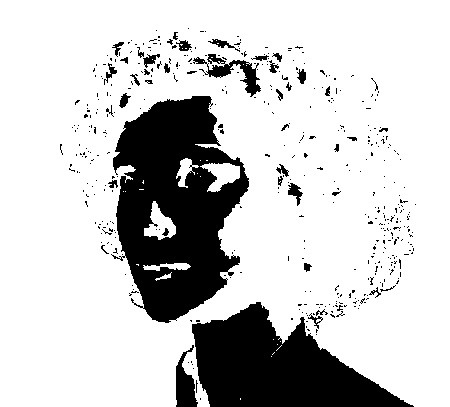
\includegraphics[width=0.25\textwidth]{img/histo/hsv/6.jpg}\label{fig:f1}}
  \subfloat[rgb]{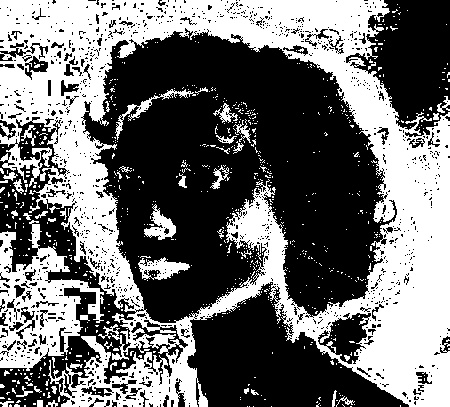
\includegraphics[width=0.25\textwidth]{img/histo/rgb/6.jpg}\label{fig:f1}}
  \subfloat[lab]{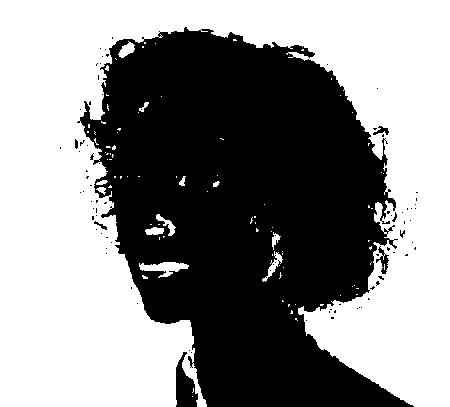
\includegraphics[width=0.25\textwidth]{img/histo/lab/6.jpg}\label{fig:f1}}

  \caption{Résultats avec histogrammes}
\end{figure}

\begin{figure}[h!]
  \centering
  \subfloat[orignal]{\includegraphics[width=0.25\textwidth]{img/histo/ori/11.jpg}\label{fig:f1}}
  \subfloat[hsv]{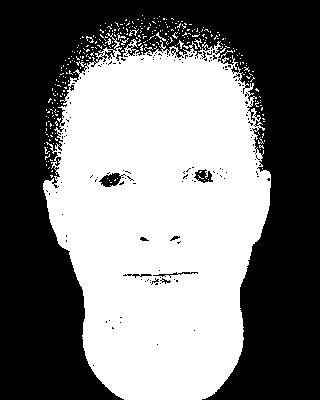
\includegraphics[width=0.25\textwidth]{img/histo/hsv/11.jpg}\label{fig:f1}}
  \subfloat[rgb]{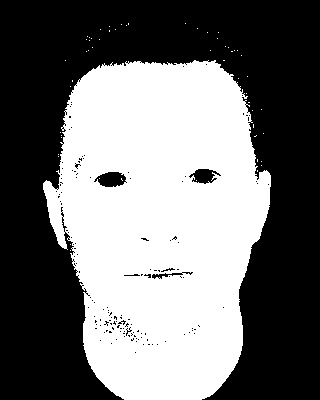
\includegraphics[width=0.25\textwidth]{img/histo/rgb/11.jpg}\label{fig:f1}}
  \subfloat[lab]{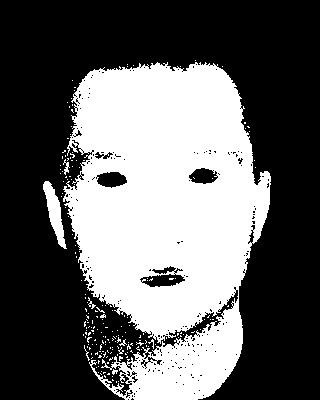
\includegraphics[width=0.25\textwidth]{img/histo/lab/11.jpg}\label{fig:f1}}

  \caption{Résultats avec histogrammes}
\end{figure}

\begin{figure}[h!]
  \centering
  \subfloat[orignal]{\includegraphics[width=0.25\textwidth]{img/histo/ori/15.jpg}\label{fig:f1}}
  \subfloat[hsv]{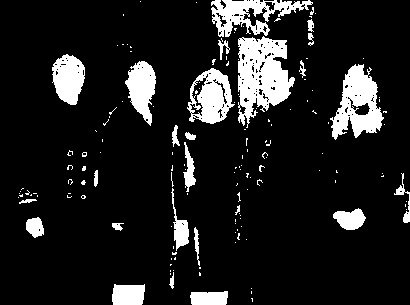
\includegraphics[width=0.25\textwidth]{img/histo/hsv/15.jpg}\label{fig:f1}}
  \subfloat[rgb]{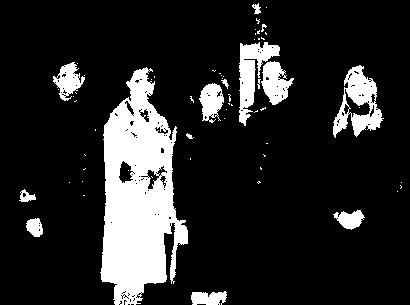
\includegraphics[width=0.25\textwidth]{img/histo/rgb/15.jpg}\label{fig:f1}}
  \subfloat[lab]{\includegraphics[width=0.25\textwidth]{img/histo/lab/15.jpg}\label{fig:f1}}

  \caption{Résultats avec histogrammes}
\end{figure}
\subsubsection{Méthode de Bayes}
J'utilise les histogrammes de la partie précédente pour mon modèle de Bayes. Pour déterminer le meilleur seuil, je cherche a maximiser le taux de bonne détection tout en minimisant celui de mauvaise détection. Pour cela, j'ai fait le choix de tester différentes valeurs de seuil en cherchant a maximiser leur différence. J'obtiens les valeurs de seuil suivante:
\begin{itemize}
    \item \textit{RGB}: $0.2$
    \item \textit{LAB}: $0.15$
    \item \textit{HSV}: $0.15$
\end{itemize}
Des seuils plus faibles permettent d'augmenter le taux de bonne détection, mais rapidement le taux de mauvaise détection grimpe au dessus des 20\%
Les résultats présentés ci dessous sont basés sur ces seuils.

\begin{table}[h!]
\centering
\resizebox{\textwidth}{!}{%
\begin{tabular}{|c|c|c|c|c|}
\hline
\multirow{2}{*}{\textbf{Dataset}} & \multicolumn{2}{c|}{\textbf{Taux de bonne détection}} & \multicolumn{2}{c|}{\textbf{Taux de mauvaise détection}} \\ \cline{2-5}
 & \textit{Moyenne} & \textit{Ecart type} & \textit{Moyenne} & \textit{Ecart type} \\ \hline
\textit{Entrainement} & 0.82 & 0.20 & 0.16 & 0.12 \\ \hline
\textit{Test} & 0.82 & 0.21 & 0.12 & 0.13 \\ \hline
\end{tabular}%
}
\caption{Résultats avec la méthode de Bayes (RGB, seuil 0.2)}
\label{bayes-rgb}
\end{table}


\begin{table}[h!]
\centering
\resizebox{\textwidth}{!}{%
\begin{tabular}{|c|c|c|c|c|}
\hline
\multirow{2}{*}{\textbf{Dataset}} & \multicolumn{2}{c|}{\textbf{Taux de bonne détection}} & \multicolumn{2}{c|}{\textbf{Taux de mauvaise détection}} \\ \cline{2-5}
 & \textit{Moyenne} & \textit{Ecart type} & \textit{Moyenne} & \textit{Ecart type} \\ \hline
\textit{Entrainement} & 0.74 & 0.26 & 0.12 & 0.11 \\ \hline
\textit{Test} & 0.73 & 0.28 & 0.08 & 0.10 \\ \hline
\end{tabular}%
}
\caption{Résultats avec la méthode de Bayes (LAB, seuil 0.15)}
\label{bayes-lab}
\end{table}


\begin{table}[h!]
\centering
\resizebox{\textwidth}{!}{%
\begin{tabular}{|c|c|c|c|c|}
\hline
\multirow{2}{*}{\textbf{Dataset}} & \multicolumn{2}{c|}{\textbf{Taux de bonne détection}} & \multicolumn{2}{c|}{\textbf{Taux de mauvaise détection}} \\ \cline{2-5}
 & \textit{Moyenne} & \textit{Ecart type} & \textit{Moyenne} & \textit{Ecart type} \\ \hline
\textit{Entrainement} & 0.88 & 0.15 & 0.26 & 0.21 \\ \hline
\textit{Test} & 0.91 & 0.11 & 0.22 & 0.16 \\ \hline
\end{tabular}%
}
\caption{Résultats avec la méthode de Bayes (HSV, seuil 0.15)}
\label{bayes-hsv}
\end{table}

\newpage
\begin{figure}[h!]
  \centering
  \subfloat[orignal]{\includegraphics[width=0.25\textwidth]{img/bayes/ori/6.jpg}\label{fig:f1}}
  \subfloat[hsv]{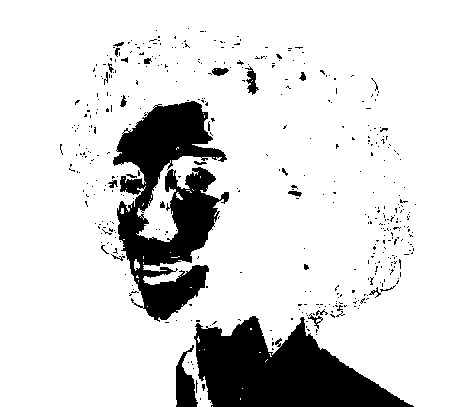
\includegraphics[width=0.25\textwidth]{img/bayes/hsv/6.jpg}\label{fig:f1}}
  \subfloat[rgb]{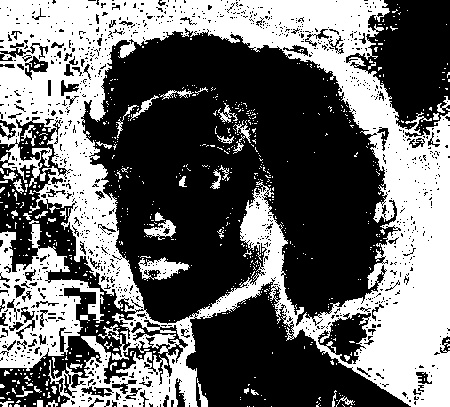
\includegraphics[width=0.25\textwidth]{img/bayes/rgb/6.jpg}\label{fig:f1}}
  \subfloat[lab]{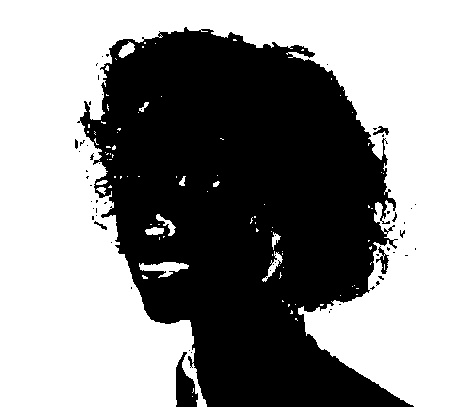
\includegraphics[width=0.25\textwidth]{img/bayes/lab/6.jpg}\label{fig:f1}}

  \caption{Résultats avec la méthode de Bayes}
\end{figure}

\begin{figure}[h!]
  \centering
  \subfloat[orignal]{\includegraphics[width=0.25\textwidth]{img/bayes/ori/11.jpg}\label{fig:f1}}
  \subfloat[hsv]{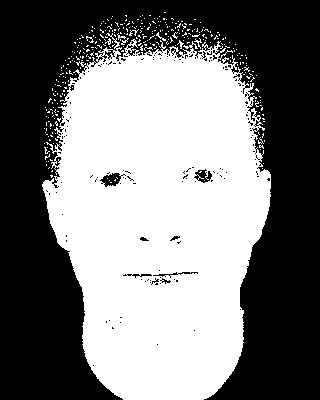
\includegraphics[width=0.25\textwidth]{img/bayes/hsv/11.jpg}\label{fig:f1}}
  \subfloat[rgb]{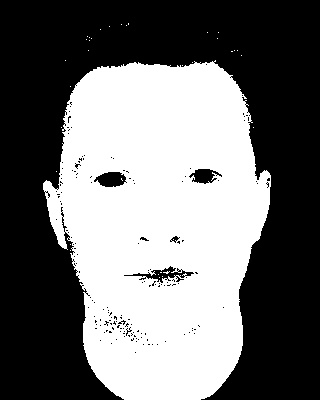
\includegraphics[width=0.25\textwidth]{img/bayes/rgb/11.jpg}\label{fig:f1}}
  \subfloat[lab]{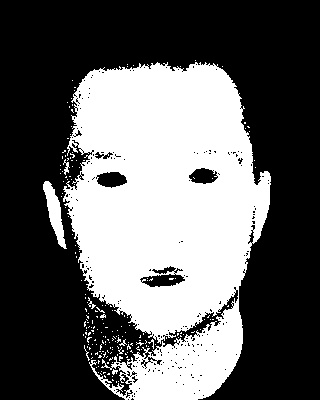
\includegraphics[width=0.25\textwidth]{img/bayes/lab/11.jpg}\label{fig:f1}}

  \caption{Résultats avec la méthode de Bayes}
\end{figure}

\begin{figure}[h!]
  \centering
  \subfloat[orignal]{\includegraphics[width=0.25\textwidth]{img/bayes/ori/15.jpg}\label{fig:f1}}
  \subfloat[hsv]{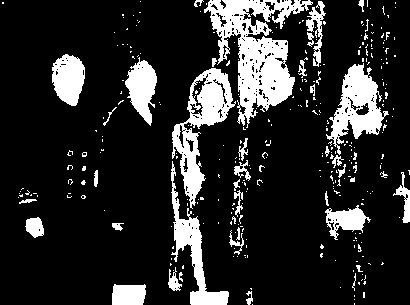
\includegraphics[width=0.25\textwidth]{img/bayes/hsv/15.jpg}\label{fig:f1}}
  \subfloat[rgb]{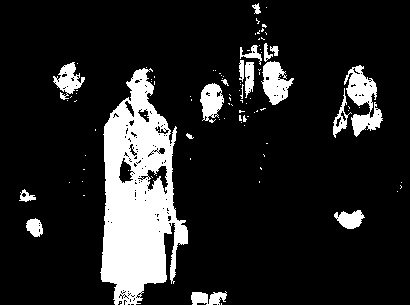
\includegraphics[width=0.25\textwidth]{img/bayes/rgb/15.jpg}\label{fig:f1}}
  \subfloat[lab]{\includegraphics[width=0.25\textwidth]{img/bayes/lab/15.jpg}\label{fig:f1}}
la méthode de Bayes
  \caption{Résultats avec la méthode de Bayes}
\end{figure}

\stepcounter{subsubsection}
\subsubsection{Discussion}

Globalement les différents modèles ont des résultats similaires. Je pense qu'il serait possible de les affiner en utilisants plus d'images différentes pour créer les histogrammes. On pourrait également affiner la qualité de la détection en combinant la détection à une recherche de contour pour détecter les visages.

\section{Detection de visages par l'approche de Viola Jones}
\subsection{Etude de la methode}
La méthode est implémenté avec les \texttt{haar cascade} de opencv. J'ai testé différents paramètres pour le detecteur. Finalement j'obtient les meilleurs résultats avec un léger scaling de l'image ($10\%$), une taille minimale de detection de 30 pixels par 30 pixels et un nombre minimal de voisin pour que la detection soit valide de 5.

\begin{figure}[h!]
  \centering
  \subfloat[]{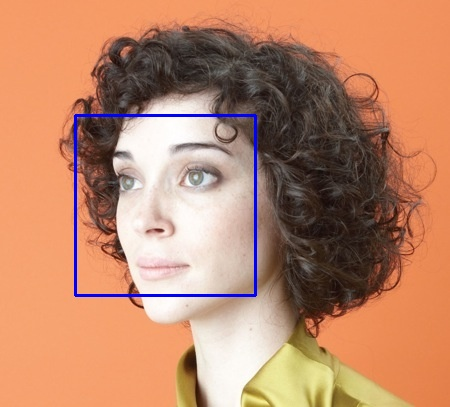
\includegraphics[width=0.4\textwidth]{img/viola/good.jpg}\label{fig:f1}}
  \hfill
  \subfloat[]{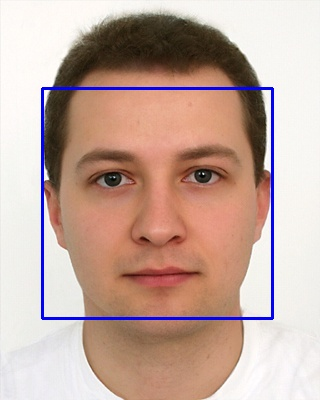
\includegraphics[width=0.4\textwidth]{img/viola/good2.jpg}\label{fig:f1}}

  \caption{Méthode de Viola Jones: exemple de bonne détection}
\end{figure}

\begin{figure}[h!]
  \centering
  \subfloat[]{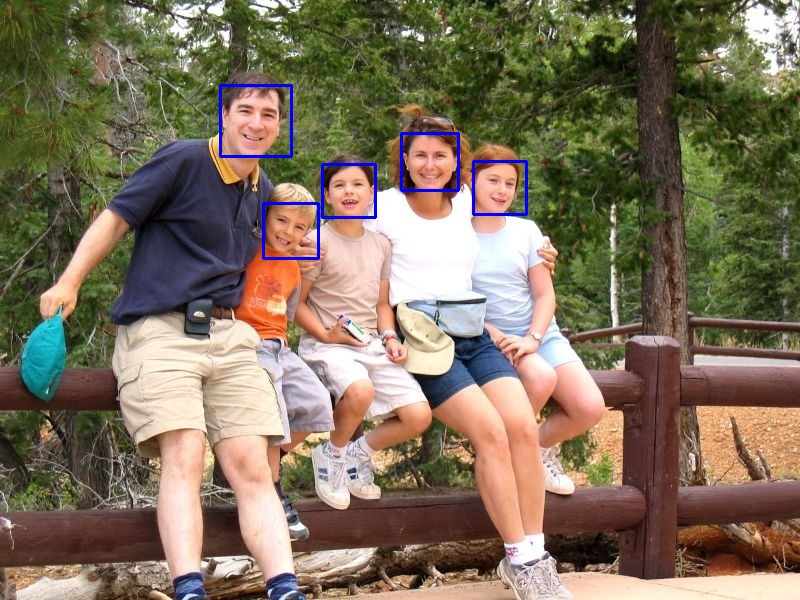
\includegraphics[width=0.4\textwidth]{img/viola/group1.jpg}\label{fig:f1}}
  \hfill
  \subfloat[]{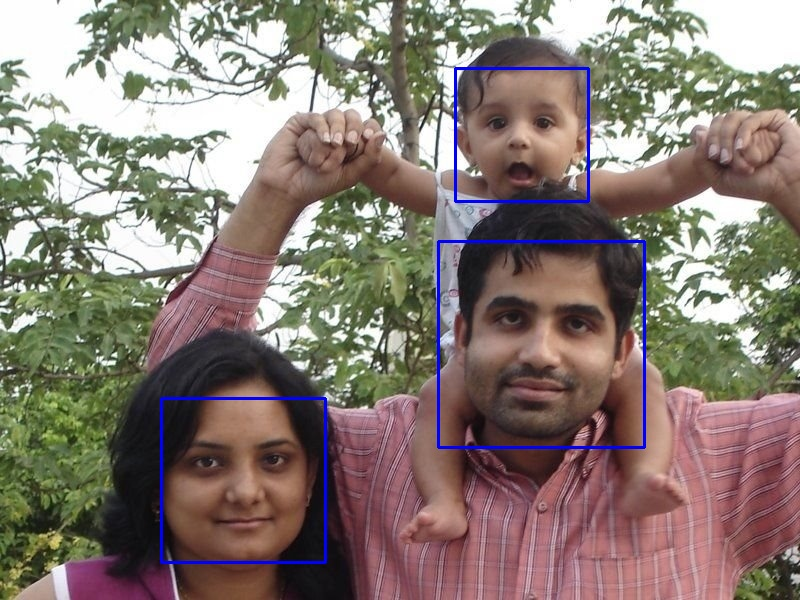
\includegraphics[width=0.4\textwidth]{img/viola/group2.jpg}\label{fig:f1}}

  \caption{Méthode de Viola Jones: exemple de bonne détection sur photo de groupes}
\end{figure}


\begin{figure}[h!]
  \centering
  \subfloat[]{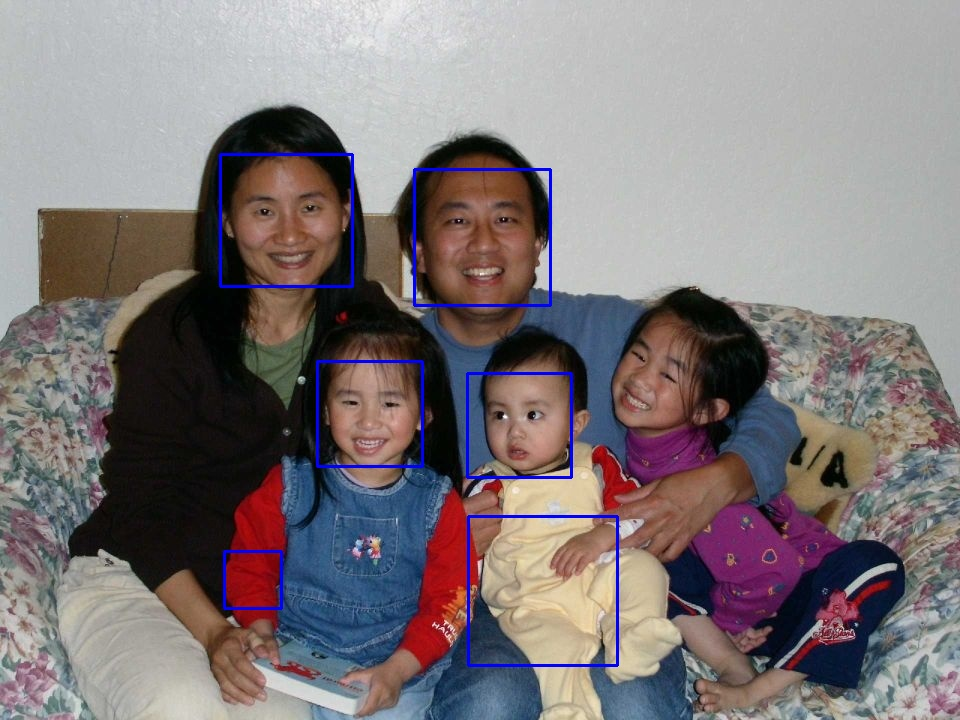
\includegraphics[width=0.4\textwidth]{img/viola/bad1.jpg}\label{fig:f1}}
  \hfill
  \subfloat[]{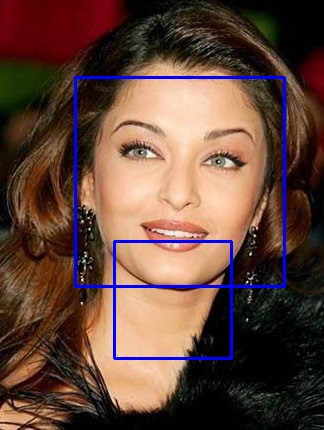
\includegraphics[width=0.4\textwidth]{img/viola/bad2.jpg}\label{fig:f1}}

  \caption{Méthode de Viola Jones: exemple de mauvaise détection}


Globalement la méthode donne de très bon résultats. Cependant comme on peux le voir dans les exemples, la détection est parfois un peu trop permitive et détecte des faux visages.
\end{figure}

\subsection{Discussion: pour aller plus loin!}
Différents articles récents présentent des modèles de détection de visage utilisant des réseaux de neuronnes profonds (\emph{deep learning}) et obtiennent de très bons résultats. \\

\\
\begin{itemize}
    \item Deep Learning Face Representation by Joint Identification-Verification - \textit{Y Sun, Y Chen, X Wang, X Tang} (2014)
    \item Deep Convolutional Network Cascade for Facial Point Detection - \textit{Yi Sun, Xiaogang Wang, Xiaoou Tang} (2013)
\end{itemize}

\end{document}
